% \documentclass[aspectratio=169,notes]{beamer}
\documentclass[aspectratio=169]{beamer}
\usetheme[faculty=phil]{fibeamer}
\usepackage{polyglossia}
\setmainlanguage{english} %% main locale instead of `english`, you
%% can typeset the presentation in either Czech or Slovak,
%% respectively.
\setotherlanguages{russian} %% The additional keys allow
%%
%%   \begin{otherlanguage}{czech}   ... \end{otherlanguage}
%%   \begin{otherlanguage}{slovak}  ... \end{otherlanguage}
%%
%% These macros specify information about the presentation
\title[MaM]{Mechanics and Machines, Lecture 12} %% that will be typeset on the
\subtitle{Overview of Strength of Materials  
\\ \   \\   
\ } %% title page.
\author{Oleg Bulichev}
%% These additional packages are used within the document:
\usepackage{ragged2e}  % `\justifying` text
\usepackage{booktabs}  % Tables
\usepackage{tabularx}
\usepackage{tikz}      % Diagrams
\usetikzlibrary{calc, shapes, backgrounds}
\usetikzlibrary{decorations.pathreplacing,calligraphy,calc,graphs}
\usepackage{amsmath, amssymb}
\usepackage{url}       % `\url`s
\usepackage{listings}  % Code listings
% \usepackage{subfigure}
\usepackage{floatrow}
\usepackage{subcaption}
\usepackage{mathtools}
\usepackage{todonotes}
\usepackage{fontspec}
\usepackage{multicol}
\usepackage{pdfpages}
\usepackage{wrapfig}
\usepackage{animate}
\usepackage{booktabs}
\usepackage{multirow}
% \usepackage{graphicx}
\usepackage{colortbl}

\graphicspath{{resources/}}
\frenchspacing

\setbeamertemplate{caption}[numbered]
\usetikzlibrary{graphs}

% \usepackage[backend=biber,style=ieee,autocite=footnote]{biblatex}
% \addbibresource{biblio.bib}
% \DefineBibliographyStrings{english}{%
%   bibliography = {References},}

\newcommand{\oleg}[2][] {\todo[color=red, #1] {OLEG:\\ #2}}
\newcommand{\fbckg}[1]{\usebackgroundtemplate{\includegraphics[width=\paperwidth]{#1}}}%frame background

\usepackage[framemethod=TikZ]{mdframed}
\newcommand{\dbox}[1]{
\begin{mdframed}[roundcorner=3pt, backgroundcolor=yellow, linewidth=0]
\vspace{1mm}
{#1}
\vspace{1mm}
\end{mdframed}
}

\begin{document}
\setlength{\abovedisplayskip}{0pt}
\setlength{\belowdisplayskip}{0pt}
\setlength{\abovedisplayshortskip}{0pt}
\setlength{\belowdisplayshortskip}{0pt}

\fbckg{fibeamer/figs/title_page.png}
\frame[c]{\setcounter{framenumber}{0}
    \usebeamerfont{title}%
    \usebeamercolor[fg]{title}%
    \begin{minipage}[b][6.5\baselineskip][b]{\textwidth}%
        \textcolor{black}{\raggedright\inserttitle}
    \end{minipage}
    % \vskip-1.5\baselineskip

    \usebeamerfont{subtitle}%
    \usebeamercolor[fg]{framesubtitle}%
    \begin{minipage}[b][3\baselineskip][b]{\textwidth}
        \raggedright%
        \insertsubtitle%
    \end{minipage}
    \vskip.25\baselineskip
}
%   \frame[c]{\maketitle}

\fbckg{fibeamer/figs/common.png}

\note{\scriptsize \begin{itemize}
        \item \
    \end{itemize}}

\begin{frame}[t]{Possible course names}
\framesubtitle{}
    \begin{columns}[T,onlytextwidth]
        \begin{column}{0.49\textwidth}
            \textbf{In Russian}
            \begin{enumerate}
                \item Сопротивление материалов (Сопромат)
                \item Техническая механика
            \end{enumerate}
        \end{column}
        \begin{column}{0.49\textwidth}
            \textbf{In English}
            \begin{enumerate}
                \item Strength of Materials
                \item Mechanics of Materials
                \item Strengths
                \item Solids
                \item Mechanics II
                \item Deformable Bodies
                \item Engineering Materials
            \end{enumerate}
        \end{column}
    \end{columns}
\end{frame}

\begin{frame}[c]{}
\framesubtitle{}
    \LARGE \centering
    Difference between theoretical mechanics and strength of material
\end{frame}

\begin{frame}[t]{Stress and Strain. Normal stress}
    \framesubtitle{Video}
    \vspace{-0.6cm}
    \begin{figure}[H]
        \href{https://youtu.be/aQf6Q8t1FQE}{
            \centering
\includegraphics[height=6cm,width=1\textwidth,keepaspectratio]{stress_video.jpg}}
        \label{fig:stress_video.jpg}
    \end{figure}
\end{frame}

\begin{frame}[t]{Stress and Strain material}
    \framesubtitle{}
    \begin{enumerate}
        \item \href{https://youtu.be/_muJSo9l18A}{Lesson 2 - Normal Stress}
        \item \href{https://youtu.be/zm-N4YQsU_M}{Normal stress notes}
        \item \href{https://youtu.be/YkdQB0JnJD4}{Simple stress and strain}
        \item \href{https://youtu.be/ywMTY8DZcsk}{Strength of Materials I: Normal and Shear Stresses (2 of 20)}
        \item \href{https://youtu.be/JB3y44-wnHQ}{Основы сопромата. Напряжения}
    \end{enumerate}
    \end{frame}

\begin{frame}[t]{Bending moment}
    \framesubtitle{Video}
    \vspace{-0.6cm}
    \begin{figure}[H]
        \href{https://youtu.be/f08Y39UiC-o}{
            \centering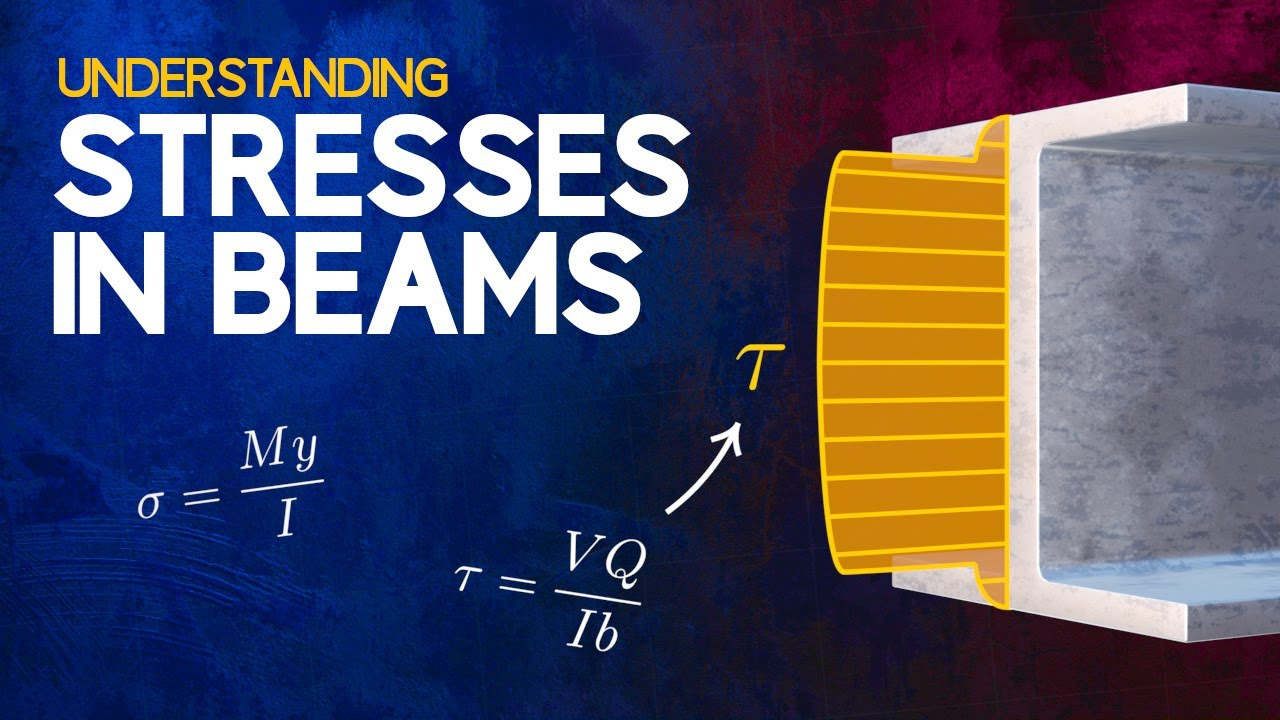
\includegraphics[height=6cm,width=1\textwidth,keepaspectratio]{bending_stress_video.jpg}}
        \label{fig:bending_stress_video.jpg}
    \end{figure}
\end{frame}

\begin{frame}[t]{Bending moment. Case study}
\framesubtitle{}
    \vspace{-0.6cm}
    \begin{figure}[H]
        \begin{subfigure}{0.49\textwidth}
            \centering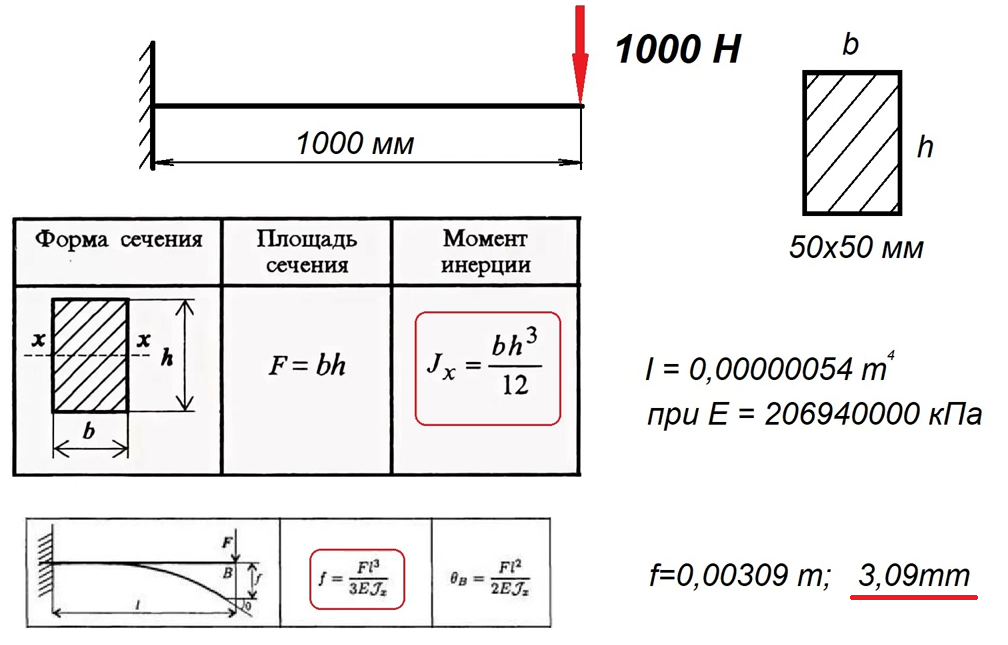
\includegraphics[height=6cm,width=1\textwidth,keepaspectratio]{task.png}
            \caption*{Analytical solution}
            \label{fig:task.png}
        \end{subfigure}
        \begin{subfigure}{0.49\textwidth}
            \centering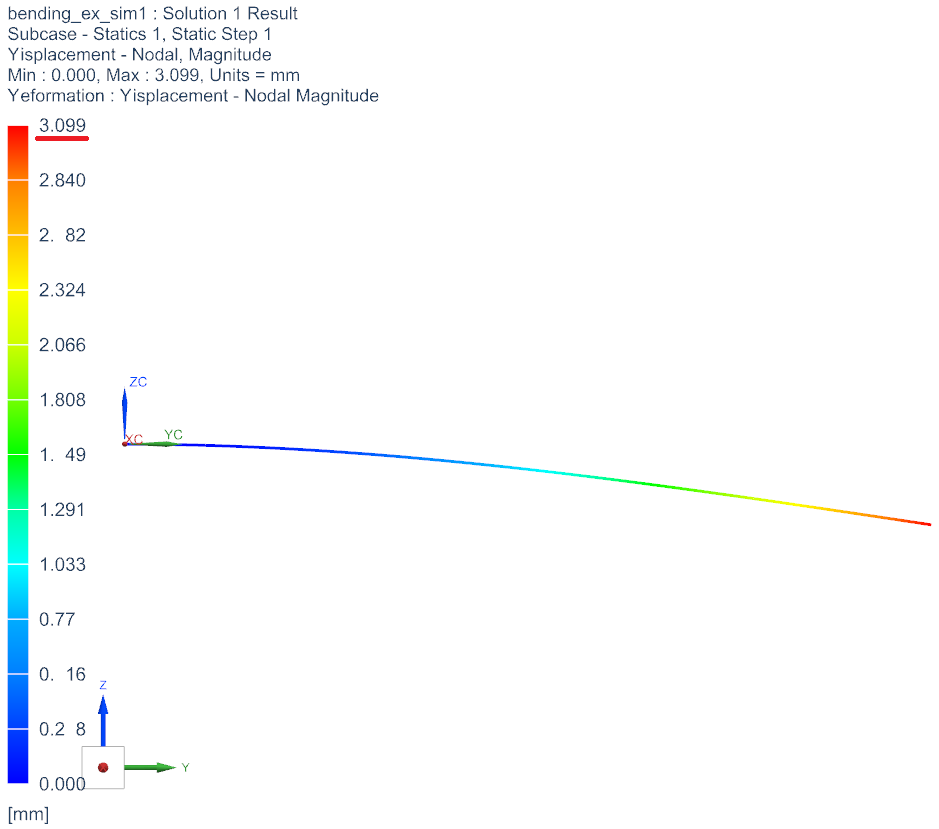
\includegraphics[height=6cm,width=1\textwidth,keepaspectratio]{bending_ex_sim1.png}
            \caption*{Numerical solution in NX}
            \label{fig:bending_ex_sim1.png}
        \end{subfigure}
    \end{figure}
\end{frame}

\begin{frame}[t]{Bending moment}
    \framesubtitle{}
    \begin{enumerate}
        \item \href{https://www.youtube.com/watch?v=1tl8SQAjWLI&list=PLOBajja3EcWJx9MVpbBvLthzmZbq4Kwlm&index=79}{Bending stress}
        \item \href{https://youtu.be/GGpTG1FSaLM}{Sign Convention For Shear Force and Bending Moment}
        \item \href{https://youtu.be/fN5np4KzIBE}{Beam bending, Shear Moment}
    \end{enumerate}
    \end{frame}

\begin{frame}[t]{Shear force}
    \framesubtitle{Video}
    \vspace{-0.6cm}
    \begin{figure}[H]
        \href{https://www.youtube.com/watch?v=wGVIRsKFqiM}{
            \centering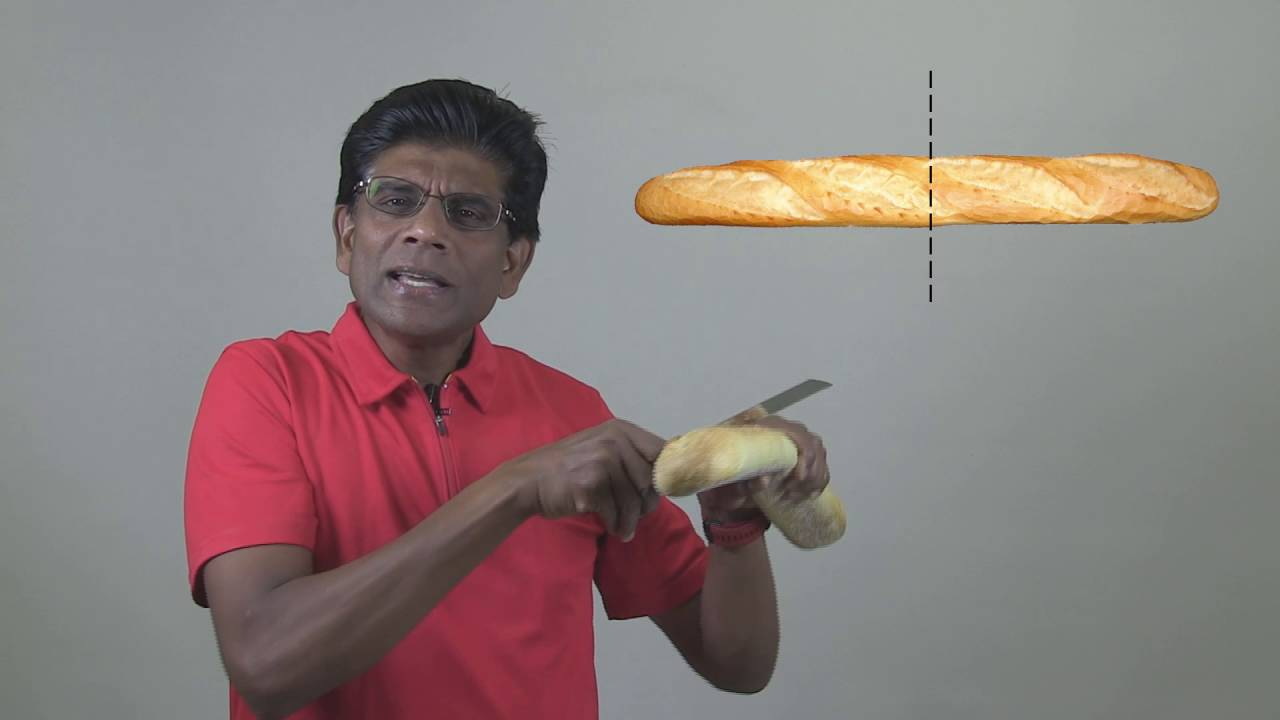
\includegraphics[height=6cm,width=1\textwidth,keepaspectratio]{shear_foce_video.jpg}}
        \label{fig:shear_foce_video.jpg}
    \end{figure}
\end{frame}

\begin{frame}[t]{Shear force material}
    \framesubtitle{}
    \begin{enumerate}
        \item \href{https://www.youtube.com/watch?v=FKu4tAaoZEM&list=PLOBajja3EcWJx9MVpbBvLthzmZbq4Kwlm&index=69&pp=iAQB}{Intro to shear}
        \item \href{https://www.youtube.com/watch?v=XlKzYy2d9BU&list=PL9RcWoqXmzaLlfmNg2Ku1SdZtvXnYrLbc&index=52&pp=iAQB}{Important concept of shear stress}
    \end{enumerate}
    \end{frame}

\begin{frame}[t]{Torsion}
    \framesubtitle{Video}
    \vspace{-0.6cm}
    \begin{figure}[H]
        \href{https://youtu.be/1YTKedLQOa0}{
            \centering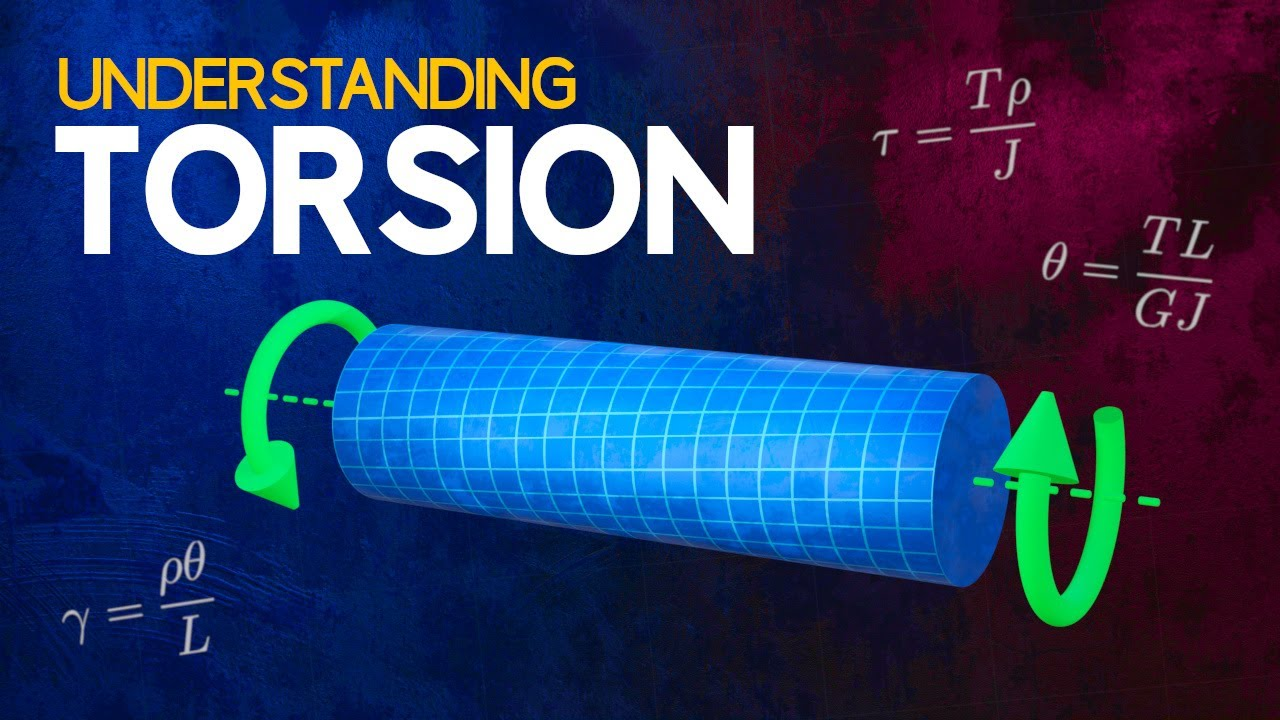
\includegraphics[height=6cm,width=1\textwidth,keepaspectratio]{torsion_video.jpg}}
        \label{fig:torsion_video.jpg}
    \end{figure}
\end{frame}

\begin{frame}[t]{Torsion material}
    \framesubtitle{}
    \begin{enumerate}
        \item \href{https://www.youtube.com/watch?v=DA75T6T5erI&list=PLZOZfX_TaWAEg1XjZ1fkUxT0XMB_Nq7hV&index=10&pp=iAQB}{Torsion in circular shaft (10 of 20)}
        \item \href{https://www.youtube.com/watch?v=HTW0PxHw_00&list=PLRqDfxcafc21wlI3E56IkDmRJ-33apMjv&index=28&pp=iAQB}{Shear stress due to torsion}
        \item \href{https://www.youtube.com/watch?v=OIYJVE7mT_4&list=PLOBajja3EcWJx9MVpbBvLthzmZbq4Kwlm&index=57&pp=iAQB}{Torsion}
    \end{enumerate}
    \end{frame}

\begin{frame}[t]{Diargams (Эпюры), Part 1}
    \framesubtitle{Video}
    \vspace{-0.6cm}
    \begin{figure}[H]
        \href{https://youtu.be/C-FEVzI8oe8}{
            \centering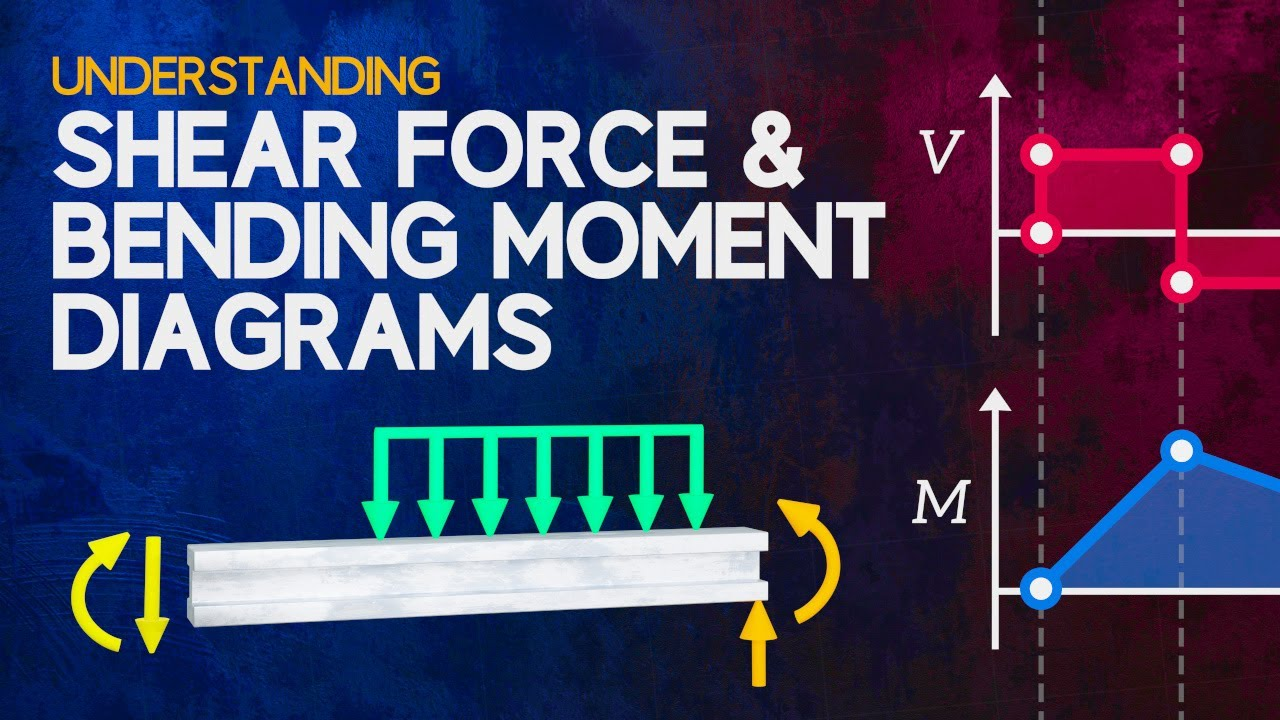
\includegraphics[height=6cm,width=1\textwidth,keepaspectratio]{diagrams1_video.jpg}}
        \label{fig:diagrams1_video.jpg}
    \end{figure}
\end{frame}

\begin{frame}[t]{Diagrams, Part 2}
    \framesubtitle{Video}
    \vspace{-0.6cm}
    \begin{figure}[H]
        \href{https://youtu.be/MvBqCeZllpQ}{
            \centering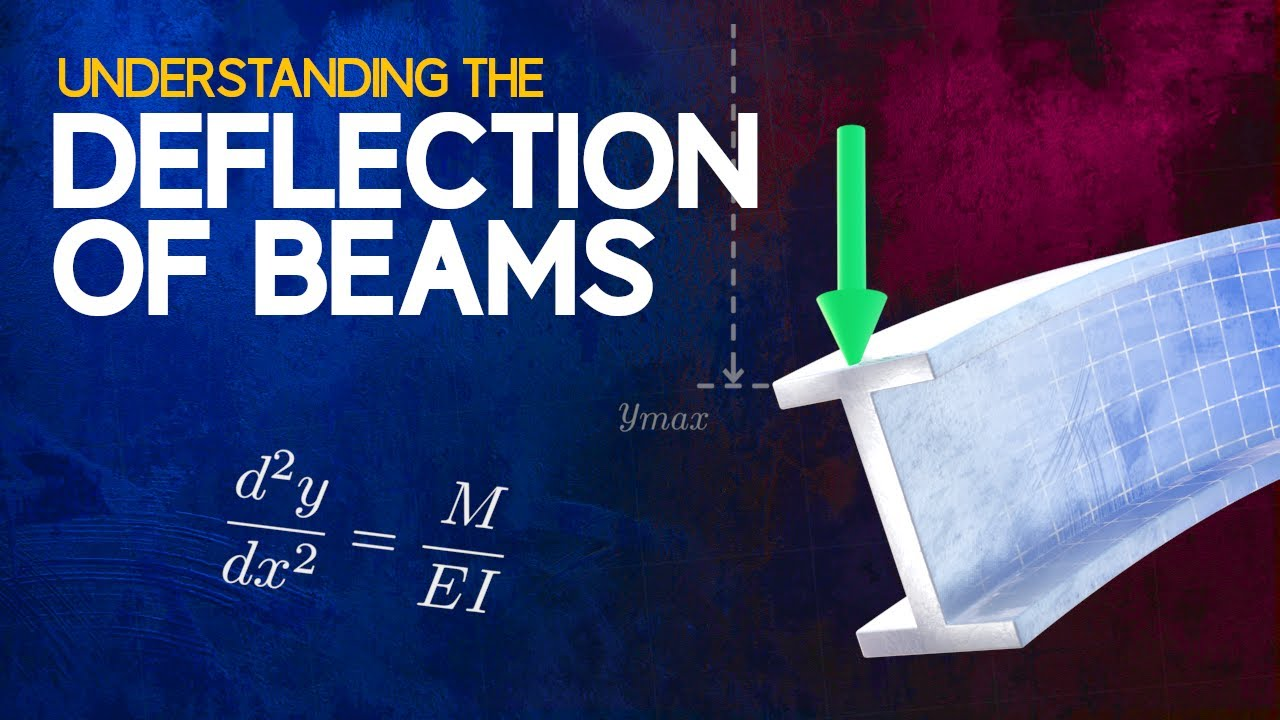
\includegraphics[height=6cm,width=1\textwidth,keepaspectratio]{diagrams2_video.jpg}}
        \label{fig:diagrams2_video.jpg}
    \end{figure}
\end{frame}

\begin{frame}[t]{Diagrams. Case study. Part 1}
\framesubtitle{}
    \vspace{-0.6cm}
    \begin{figure}[H]
        \centering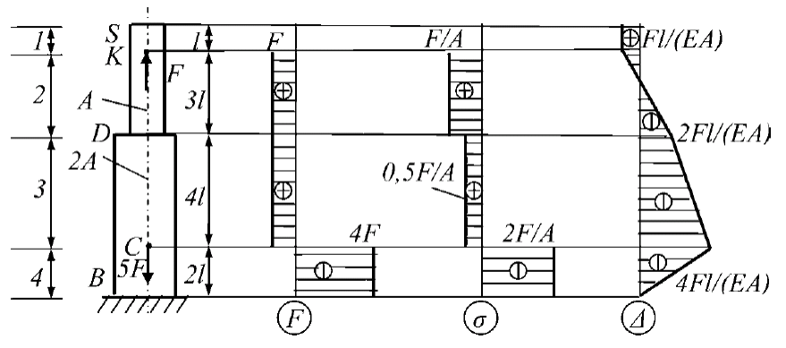
\includegraphics[height=6cm,width=1\textwidth,keepaspectratio]{diagram_task.png}
        \label{fig:diagram_task.png}
    \end{figure}
\end{frame}

\begin{frame}[t]{Diagrams. Case study. Part 2}
\framesubtitle{}
    \vspace{-0.6cm}
    \begin{figure}[H]
        \begin{subfigure}{0.59\textwidth}
            \centering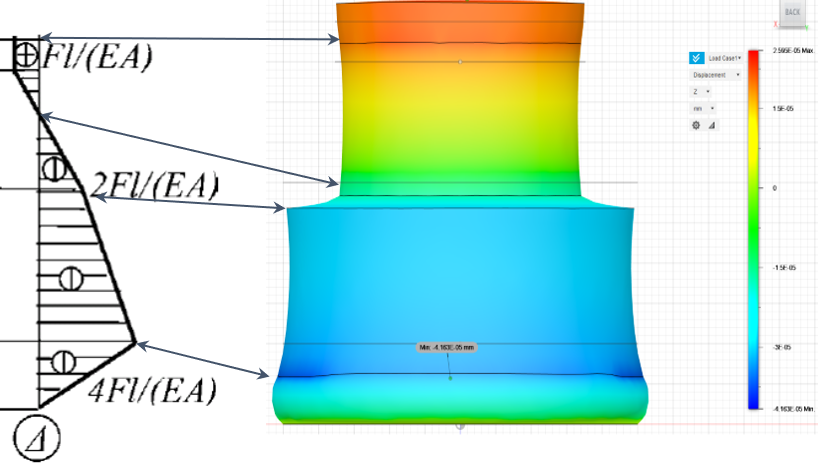
\includegraphics[height=6cm,width=1\textwidth,keepaspectratio]{fusion.png}
            \caption*{Analytical + Fusion 360}
            \label{fig:fusion.png}
        \end{subfigure}
        \begin{subfigure}{0.39\textwidth}
            \centering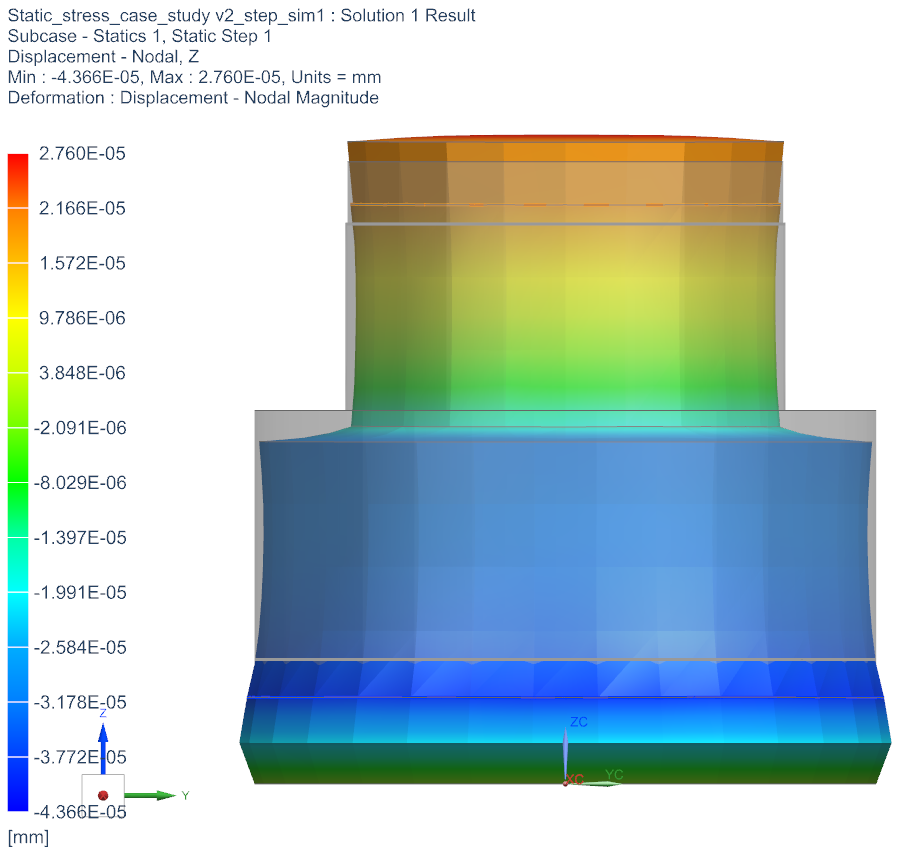
\includegraphics[height=6cm,width=1\textwidth,keepaspectratio]{Static_stress_case_study_v2_step_sim1.png}
            \caption*{Siemens NX}
            \label{fig:Static_stress_case_study_v2_step_sim1.png}
        \end{subfigure}
    \end{figure}
\end{frame}

\begin{frame}[t]{Diagrams material}
    \framesubtitle{}
    \begin{enumerate}
        \item \href{https://youtu.be/BjFghX-MScA}{Shear and bending diagrams example}
        \item \href{https://youtu.be/Kj3IKgp4020}{Эпюры}
        \item \href{https://youtu.be/hSb6NVYVl30}{How to calculate Shear Force and Bending Moment diagram ? Explained with Animation and numerical}
    \end{enumerate}
    \end{frame}

\begin{frame}[t]{Safety factor}
    \framesubtitle{Video}
    \vspace{-0.6cm}
    \begin{figure}[H]
        \href{https://www.youtube.com/watch?v=7s06qpjaUJA&list=PLRqDfxcafc21wlI3E56IkDmRJ-33apMjv&index=8}{
            \centering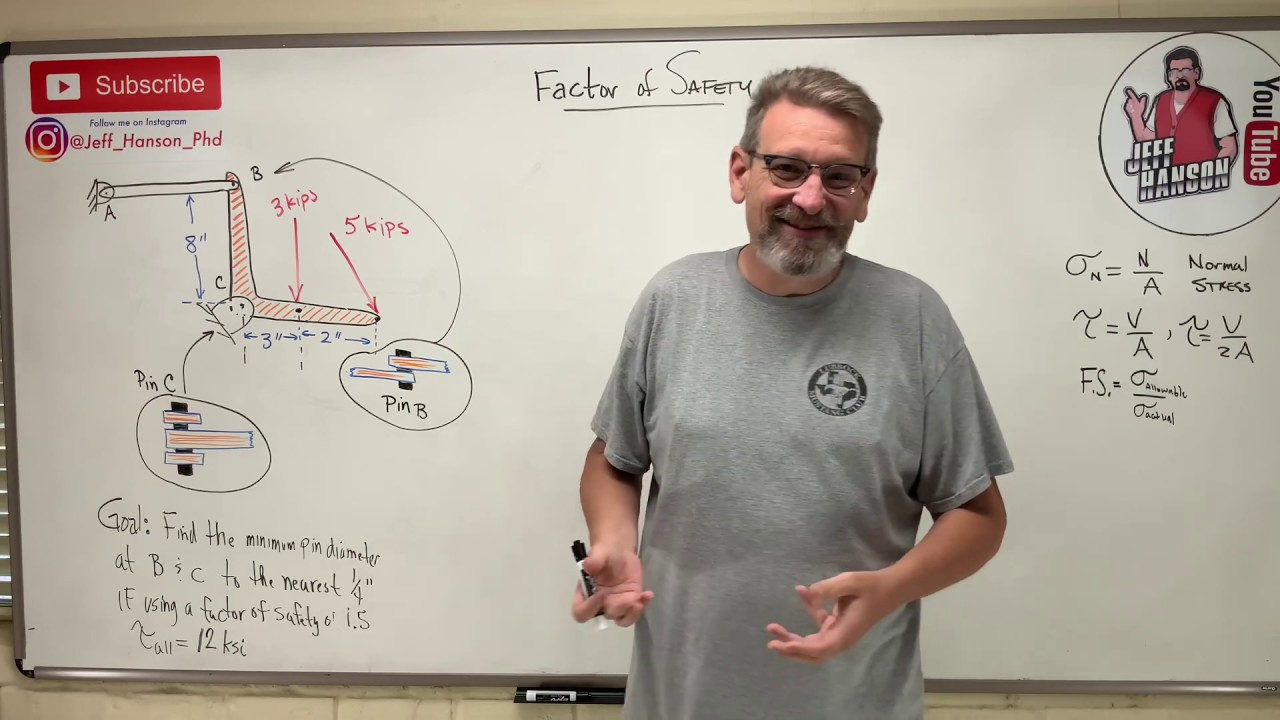
\includegraphics[height=6cm,width=1\textwidth,keepaspectratio]{safety_factor_video.jpg}}
        \label{fig:safety_factor_video.jpg}
    \end{figure}
\end{frame}

\begin{frame}[t]{Failure Theories (von Mises!)}
    \framesubtitle{Video}
    \vspace{-0.6cm}
    \begin{figure}[H]
        \href{https://youtu.be/xkbQnBAOFEg}{
            \centering
\includegraphics[height=6cm,width=1\textwidth,keepaspectratio]{failure_theories_video.jpg}}
        \label{fig:failure_theories_video.jpg}
    \end{figure}
\end{frame}

\begin{frame}[t]{Failure Theories material}
    \framesubtitle{}
    \begin{enumerate}
        \item \href{https://www.youtube.com/watch?v=QV6xB0bLJwM&list=PLRqDfxcafc21wlI3E56IkDmRJ-33apMjv&index=64&t=183s}{Lesson 55 - Tresca, Von Mises, and Rankine Failure Theories Explained}
    \end{enumerate}
    \end{frame}

\begin{frame}[t]{Reference Material (playlist)}
    \framesubtitle{}
    \begin{enumerate}
        \item \href{https://www.youtube.com/playlist?list=PLOBajja3EcWJx9MVpbBvLthzmZbq4Kwlm}{Mechanics of Material (math) (video)}
        \item \href{https://www.youtube.com/playlist?list=PL9RcWoqXmzaLlfmNg2Ku1SdZtvXnYrLbc}{Strength of Materials (lecture-like)}
        \item \href{https://www.youtube.com/playlist?list=PLRqDfxcafc21wlI3E56IkDmRJ-33apMjv}{Mechanics of Solids (small whiteboard videos)}
        \item \href{https://www.youtube.com/playlist?list=PLEYqyyrm-hQ3wtF34smyJSAOqUJqnf1ch}{Mechanics of Materials (fancy animation)}
        \item \href{https://www.youtube.com/playlist?list=PLZOZfX_TaWAEg1XjZ1fkUxT0XMB_Nq7hV}{Strength of Materials Dr. IZadi}
        \item \href{https://www.youtube.com/playlist?list=PLFOi9-wTdZsP1SdgG2qok-2gOyhgKilX7}{Основы сопромата}
        \item "Mechanics of Materials" by Russell C Hibbeler
        \item Писаренко Г.С., Яковлев А.П., Матвеев В.В. Справочник по сопротивлению материалов 1988
        \item Тимошенко С.П. Сопротивление материалов. 1965
    \end{enumerate}
    \end{frame}

\fbckg{fibeamer/figs/last_page.png}
\frame[plain]{}

\end{document}